\documentclass[11pt, letterpaper]{article}
\usepackage{palatino}
\usepackage{graphicx}
\usepackage{enumitem}
\usepackage[top=1in, left=1in, right=1in, bottom=1in]{geometry}

\begin{document}
\begin{center}
\Large{\textbf{Audio Language Classifier:}}

\Large{\textbf{Model Metrics}}

\large{Kirsten Regier}
\end{center}


\section{Gender classifier}
\subsection{Model structure}

Two different models were trained and evaluated for the gender classifier. The structure of each model is shown in Table \ref{tab:GenModels}. 

The models had identical input and output layers. The shape of the input was (32, 10, 128), which corresponds to the batch size (32) and the VGGish embedding (10, 128).  Since the classification was binary, the output layer contained one node, with a sigmoid activation function.

The models differ in the number of hidden layers. Each hidden layer consisted of a dense layer followed by a dropout layer with a dropout rate of 50\%. The first model contained a single hidden layer with 128 nodes. The second model contained two hidden layers, the first with 128 nodes, and the second with 64 nodes. Prior to being fed into the output layer, the output from the previous layer was flattened into a 1D array. The shape of the flattened array varied for each model, based on the number of nodes of the prior layer (128 vs 64).

\begin{table}[!h]
\begin{center}
\caption{Structure of the two gender classifier models. Model 1 has one hidden layer with 128 nodes, while Model 2 has two hidden layers with 128 and 64 nodes, respectively.}
\begin{tabular}{l | c | c |}

Layer  & Model 1 & Model 2\\
\hline

Input 	& (32, 10, 128) & (32, 10, 128) \\ \hline

Dense	& 128 nodes & 128 nodes \\
Dropout	& 50\%		& 50 \% \\ \hline

Dense	&			& 64 nodes \\
Dropout	& 			& 50\% \\ \hline

Flatten 	& (32, 1280)	& (32, 640) \\ \hline
Output 	& (32, 1)		& (32, 1)\\
\hline
\end{tabular}

\label{tab:GenModels}
\end{center}
\end{table}

\subsection{Training time}

Each model was set to run for 100 epochs, or until the validation loss stopped decreasing for 5 consecutive epochs. Model 1 trained for 8 epochs, with the lowest validation loss found at epoch 3. Model 2 trained for 7 epochs, with the lowest validation loss at epoch 2. The evaluation metrics below are based on the weights of the models with the lowest validation loss - after epochs 3 and 2, respectively.

\subsection{Model evaluation}

As shown in Table \ref{tab:GenConfusion}, both models performed quite well on the binary classification task, reaching an accuracy of 98.14\% and 97.55\%, respectively. Model 1 showed similar performance between both classes, with nearly equal numbers of speakers being misclassified from each class. Model 2 showed more discrepancies between the performance of the two classes. Male voices were identified correctly at a rate of 99.14\%, while female voices were identified correctly only 96.5\%. However, the precision of the predictions was the reverse - the precision of female voice prediction was 99.14\%, while the precision of male voice prediction was 96.02\%.

\begin{table}[h]
\begin{center}
\caption{Confusion Matrices for the Gender Classifier Models}
\begin{tabular}{l l | c c r }
\multicolumn{2}{l}{\textbf{Model 1}} & \multicolumn{2}{c}{Predicted} & Recall \\
& & F & M &  \\ 
\cline{2-5}
Actual & F & 590 &  10 & 0.9833 \\
& M & 12 & 572 & 0.9795 \\  \hline
Precision&  & 0.9801 & 0.9828 \\ 
Accuracy & & &  & 0.9814 \\
\end{tabular}
\begin{tabular}{l l | c c r }
\multicolumn{2}{l}{\textbf{Model 2}} & \multicolumn{2}{c}{Predicted} & Recall \\
& & F& M &  \\ 
\cline{2-5}
Actual & F & 576 &  24 & 0.9650 \\
& M & 5 & 579 & 0.9914 \\  \hline
Precision&  & 0.9914 & 0.9602 \\ 
Accuracy & & &  & 0.9755 \\
\end{tabular}
\label{tab:GenConfusion}
\end{center}
\end{table} 

\begin{table}[h]
\begin{center}
\caption{Gender Classifiers - Metrics summary}
\begin{tabular}{l c c}
& 	Model 1 & Model 2 \\ \hline
loss	&0.061640 & 0.076962 \\
accuracy& 0.981419 & 0.975507 \\
precision & 0.982818 & 0.960199 \\
recall & 0.979452 & 0.991438 \\
\end{tabular}
\label{tab:GenMetricsSum}
\end{center}
\end{table} 

Given the slightly better accuracy rates, and the more consistent values of precision and recall between the two classes, it seems that the simpler, one layer model performs slightly better than the more complex, two-layered model for general use cases.

%make up  a story about when to use model one and two based on difference in recall and precision
%- diagnosis vs X
%- minimize false positives
%- use cases for recall (sensitivity) vs precision.

% Screening vs diagnosis
% - screening = find early, non-symptomatic cases in general population
% - diagnosis = find out exactly what is wrong in symptomatic cases

Model 1 has similar rates of mis-categorizing both male and female voices. About the same number of male voices are identified as female as female voices that are identified as male. Likewise, roughly the same percentage of voices identified as female are actually female and identified as male are actually male. (Roughly equal sensitivity, specificity and precision, roughly equal positive predictive value and negative predicted value).

Model 2 has higher sensitivity for male voices and lower specificity for female voices.
If you expect most of the callers to be male, if the cost is low for misidentifying females as males,

Model 2 - better sensitivity (recall) for male voices [ but worse specificity for female voices] - identifies male voices as male most of the time; better precision for female voices - fewer predicted female voices were not female. 
Model 2 has high sensitivity  for male voices, but lower specificity of female voices.  Higher precision for female voices ( more cases predicted female are actually female, fewer cases predicted male are actually male.) More likely to categorize a female voice as male than a male voice as female.
Model 2 rarely mis-categorizes a male voice as female, but more frequently mis-categorizes a female voice as male. If the model predicts female, the voice is more likely to be female; if the model predicts male, there is slightly less of a chance that the voice is actually male. However, if the voice is actually male, it is more likely that it will be categorized correctly. %If you expect to have mostly male callers, it does a good job identifying them; if you expect mostly female callers, it will have a higher miss rate.

\section{Language classifier}
\subsection{Model structure}

Several different models were trained and evaluated for the language classifier. The structure of each model is shown in Table \ref{tab:LangModels}. 

All of the models had identical input and output layers. The shape of the input was (32, 10, 128), which corresponds to the batch size (32) and the VGGish embedding (10, 128).  There were 11 possible classes, so the output layer consisted of 11 nodes. A softmax activation function was used on the output layer, so that the output vector contained the probability that the speaker belonged to each of the output classes. The class with the highest probability was take to the be predicted class.

The models differ in the number of nodes and the number of hidden layers. Each hidden layer consisted of a dense layer followed by a dropout layer with a dropout rate of 50\%. The first model contained a single hidden layer with 12 nodes, while the second model had a single layer with 128 nodes. The third model contained two hidden layers, the first with 128 nodes, and the second with 64 nodes. Prior to being fed into the output layer, the output from the previous layer was flattened into a 1D array. The shape of the flattened array varied for each model, based on the number of nodes of the prior layer (12 vs 128 vs 64).

\begin{table}[!h]
\begin{center}
\caption{Structure of the language classifier models. Model 1 has one hidden layer with 12 nodes, Model 2 has one hidden layer with 128 nodes, and Model 3 has two hidden layers with 128 and 64 nodes, respectively.}
\begin{tabular}{l | c |c  | c |}

Layer  & Model 1 & Model 2 & Model 3\\
\hline

Input 	& (32, 10, 128)& (32, 10, 128) & (32, 10, 128) \\ \hline

Dense	& 12 nodes 	& 128 nodes 	& 128 nodes \\
Dropout	& 50\%		& 50\%		& 50 \% \\ \hline

Dense	&			&			& 64 nodes \\
Dropout	&			& 			& 50\% \\ \hline

Flatten 	& (32, 120)	& (32, 1280)	& (32, 640) \\ \hline
Output 	& (32, 11)		& (32, 11)		& (32, 11)\\
\hline
\end{tabular}

\label{tab:LangModels}
\end{center}
\end{table}

\subsection{Training time}

Each model was set to run for 100 epochs, or until the validation loss stopped decreasing for 5 consecutive epochs. Models 1 and 3 each trained for 12 epochs, with the lowest validation loss found at epoch 7. Model 2 trained for 9 epochs, with the lowest validation loss at epoch 4. 

For Model 1, the evaluation metrics reported below are based on the model weights after epoch 7 (the best weights), whereas for Models 2 \& 3, the metrics are based on the model weights after the final training epoch.

\subsection{Model evaluation}
\subsubsection{Baseline calculations}

The dataset contained many more speakers of English, Spanish and Arabic than speakers of other languages. To balance the classes for the Language Classifier, the number of speakers for these languages was downsampled to 75, which meant that each of these language classes contained 12.0773\% of the total number of speakers in the dataset. German had the fewest number of speakers (36), which comprised 5.797\% of the data. The distribution of the number of \textbf{speakers} sampled per language class is shown in blue in Figure \ref{fig:LangDistTot}. The speakers of each language were split into training, validation and testing sets, so the distribution of speakers in each data split reflects the overall distribution of speakers, as shown in the left panel of Figure \ref{fig:LangDist}.

\begin{figure}[h]
\begin{center}
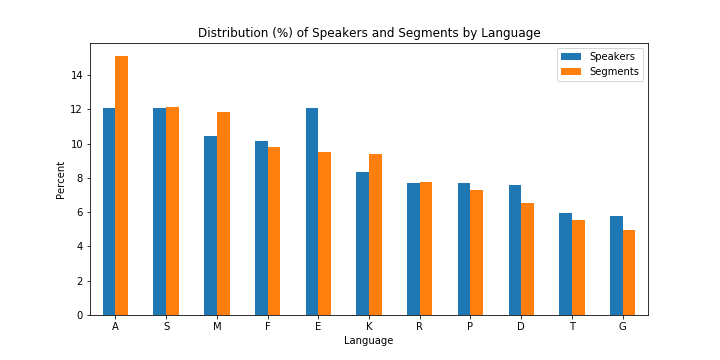
\includegraphics[width=6in]{LangDistPercentSpSeg.png}
\caption{Distribution of Speakers and Segments by Language}
\label{fig:LangDistTot}
\end{center}
\end{figure}

After the speakers were assigned to the data splits, the audio files for all speakers were segmented, and the segments in the training and validation splits were augmented with noise. Since the number of segments per speaker was dependent on the length of the original audio file, which was not determined before the speakers were split, the number of segments per language and per data split were not identical to the distribution of the speakers. While the distribution of speakers and segments for most of the languages remains similar (compare the heights of the blue and orange bars in Figure \ref{fig:LangDistTot}), the distribution of Arabic and English segments changed dramatically. While there were equal numbers of Arabic and English speakers (75 per language, or 12.07\% each), there were 380 Arabic segments and 138 English segments. Thus, the Arabic segments represented 15.741508\% of the segments, while the English segments represented only 5.716653\% of segments. Furthermore, as shown in the right panel of Figure \ref{fig:LangDist}, the English segments comprised 9.9196\% of the testing data, which is roughly double their distribution in the training and validation sets, which were 5.0360\% and 4.6875\%, respectively.

\begin{figure}[h]
\begin{center}
\includegraphics[width=6in]{PctSpSegbyLangperSplit.png}
\caption{Distribution of Speakers and Segments by Language}
\label{fig:LangDist}
\end{center}
\end{figure}

\subsection{Model Metrics}
Arabic has the greatest number of segments in the dataset, with 15.7\% of the segments. The smallest language class was German, with 125 segments (5.178128\%). A naive classifier that always predicted the majority class (Arabic) would have an accuracy of 15.7\%.  All three of the models improved upon this baseline accuracy rate, as shown in the second row of Table \ref{tab:LangMetricsSum}. Based on the metrics presented in Table \ref{tab:LangMetricsSum}, Model 3 is the best performing model in terms of loss, accuracy, and F1 score (all versions).

\begin{table}[h]
\begin{center}
\caption{Language Classifiers - Metrics summary}
\begin{tabular}{l c c c}
& 	Model 1 & Model 2 & Model 3\\ \hline
loss	&2.300652266 & 2.353183508 & 2.283754587 \\
accuracy& 0.178977266 & 0.23011364 &  0.241477266\\
precision & 1 & 0.460317463 & 0.649999976\\
recall & 0.002840909 & 0.082386367 & 0.082386367\\
F1 score micro & 0.178977273 & 0.230113636  & 0.241477273\\
F1 score macro & 0.084855919 & 0.169606263 & 0.171586068 \\
F1 score weighted & 0.122333655 & 0.193686198 & 0.202591296 \\
\end{tabular}
\label{tab:LangMetricsSum}
\end{center}
\end{table} 

The confusion matrix for the Model 3 predictions is shown in Table \ref{tab:LangConfMat}. Not surprisingly, the class with the highest correct predictions was the majority class, Arabic, at 28. Mandarin and Dutch also had relatively high correct predictions at 18 and 17, respectively. German, the smallest class, and Russian showed no correct predictions, while Turkish and Portuguese each had a single correct prediction.

Behind Arabic, Mandarin and Spanish contributed about the same number of segments to each of the training sets (12.344656\% and12.676056 \%, respectively). While there were more predictions for Mandarin (73) than Spanish (27), and more correctly classified Mandarin samples (18) than Spanish (6), the precision rates for the two classes was similar at .25 for Mandarin and .22 for Spanish.

Dutch is really interesting - there were relatively few Dutch samples, but Dutch was predicted 3rd most often (behind Arabic and Mandarin), and was also third highest in number of correct predictions.

Other "common" confusions:
Korean as Arabic - 12
Arabic as Dutch - 10
Arabic as Mandarin - 12

Related languages -  that might be similarly confused
English vs Dutch - 2 D as E, 6 E as D
Eng vs German - 0 E as G, 4 G as E
Dutch vs German - 0 D as G, 1 G as D

Span vs port.
2 S as P; 1 P as S
7 P as F; 6 F as P
4 S as F; 4 F as S


\begin{table}
\begin{center}
\caption{Confusion matrix for Model 3 predictions. The bold numbers on the diagonal represent correct predictions.}
\begin{tabular}{l | c c c c c c c c c c c || c}

lang   & R &A &T &K &G &D &S &F &E &P &M & Segments\\ \hline
Russian   & \textbf{0} &6 &3 &1 &0 &3 &0 &2 &1 &4 & 8 & 28\\ % russian
Arabic   & 0 &\textbf{28} &1 &0 &1 &10 &1 &0 &2 &0 &12 & 55\\ % arabic
Turkish   & 0 &3 &\textbf{1} &0 &0 &4 &5 &1 &2 &1 &4 & 21\\ % turkish
Korean   & 0 &12 &0 &\textbf{2} &0 &6 &1 &1 &2 &2 &5 & 31 \\ % korean
German   & 0 &2 &0 &1 &\textbf{0} &1 &4 &1 &4 &2 &0 &15 \\ % german
Dutch   & 0 &1 &0 &0 &0 &\textbf{17} & 1 & 0 & 2 & 2 & 2 & 25 \\ % dutch
Spanish   & 2 &7 &0 &1 &4 &3 &\textbf{6} &4 &6 &2 &7& 42\\ % spanish
French   & 0 &9 &0 &0 &0 &4 &4 &\textbf{3} &0 &6 &6 & 32\\ % french
English   & 0 &2 &0 &1 &0 &6 &1 &5 &\textbf{9} &0 &6 & 30\\ % english
Portuguese   & 0 &8 &1 &0 &1 &2 &1 &7 &2 &\textbf{1} &5 & 28\\ % portuguese
Mandarin & 1 &2 &3 &2 &0 &5 &3 &3 &2 &6 &\textbf{18} & 45 \\ \hline % mandarin
\hline
Total & 3 & 80 & 9 & 8  & 6 & 61 & 27 & 27 & 32 & 26  & 73 &  352

\end{tabular}
\label{tab:LangConfMat}
\end{center}
\end{table}

Classification report

\begin{table}
\begin{center}
\caption{Metrics (precision, recall and F1 score) by language class}
\begin{tabular}{l c c c c}
language  &   precision &   recall  &f1-score &  support \\ \hline

Russian	&  0.00    &  0.00   &   0.00    &    28  \\
Arabic    &   0.35    &  0.51   &   0.41    &    55\\ 
Turkish    &   0.11    &  0.05   &   0.07    &    21\\
Korean    &   0.25   &   0.06  &    0.10   &     31\\
German  &     0.00 &     0.00  &    0.00  &      15\\
Dutch    &   0.28   &   0.68   &   0.40    &    25\\
Spanish  &     0.22 &     0.14   &   0.17  &      42\\
French   &    0.11   &   0.09    &  0.10    &    32\\
English   &    0.28  &    0.30   &   0.29   &     30\\
Portuguese &      0.04  &    0.04  &    0.04   &     28\\
Mandarin   &    0.25    &  0.40   &   0.31    &    45\\ \hline

Accuracy      &         &         &   0.24  &     352\\
Macro avg     &  0.17   &   0.21    &  0.17     &  352\\
Weighted avg    &   0.20    &  0.24     & 0.20     &  352\\ \hline
\end{tabular}
\end{center}
\end{table}



Model metrics for all models

15.7\% of segments were Arabic - majority class in segment data.

\end{document}


Accuracy keeps increasing; future work add more layers, add complexity to model.